\documentclass[11pt,a4paper]{article}

\usepackage[margin=2.4cm]{geometry}
\usepackage{amsmath}
\usepackage{fontspec}
\usepackage{unicode-math}
\setmainfont{Times New Roman}
\setmathfont{texgyretermes-math.otf}
\usepackage{setspace}
\setstretch{1.12}
\usepackage{microtype}
\usepackage{graphicx}
\usepackage{booktabs}
\usepackage{tabularx}
\usepackage{adjustbox}
\usepackage{float}
\usepackage{multirow}
\usepackage{array}
\usepackage{enumitem}
\usepackage{xcolor}
\usepackage{caption}
\usepackage{tikz}
\usetikzlibrary{positioning,arrows.meta,shapes.misc}
\usepackage[hidelinks]{hyperref}
\hypersetup{pdftitle={Detecting AI Generated Images Across Generators}, pdfauthor={Group 135: Choi Seunghwan, Tyrone Tiang Jin Shen, Michael Yip Hoi Weng}}

\definecolor{ntublue}{HTML}{181C62}
\definecolor{ntured}{HTML}{D71440}
\captionsetup{font=small,labelfont=bf}
\setlist{itemsep=2pt,topsep=4pt}
\newcolumntype{R}{>{\raggedleft\arraybackslash}X}
\newcommand{\best}[1]{\textbf{#1}}
\newcommand{\pp}{\,pp}
\newcommand{\why}[1]{\noindent\textit{\color{ntublue}Motivation.} #1\par\smallskip}
\newcommand{\ledto}[1]{\par\smallskip\noindent\textit{\color{ntublue}What it led to.} #1\par}

\begin{document}

% ------------------------------------------------------------------ cover
\begin{titlepage}
  \centering
  \vspace*{0.5cm}
  
\includegraphics[width=0.62\textwidth]{figures/ntu_logo.png}\par
  \vspace{2.2cm}
  {\large\color{ntublue} SC4001 Neural Networks and Deep Learning\par}
  \vspace{0.3cm}
  {\large Group Project Report, Direction J\par}
  \vspace{0.3cm}
  {\large\bfseries Group 135\par}
  \vspace{1.6cm}
  {\color{ntured}\rule{0.8\textwidth}{0.8pt}\par}
  \vspace{0.6cm}
  {\LARGE\bfseries Detecting AI Generated Images Across Generators\par}
  \vspace{0.6cm}
  {\color{ntured}\rule{0.8\textwidth}{0.8pt}\par}
  \vspace{2.2cm}
  {\large
  \renewcommand{\arraystretch}{1.6}
  \begin{adjustbox}{max width=\textwidth}\begin{tabular}{l@{\hspace{2.5cm}}l}
    \textbf{Name} & \textbf{Matriculation No.} \\
    \hline
    Choi Seunghwan & U2021319B \\
    Tyrone Tiang Jin Shen & U2420849F \\
    Michael Yip Hoi Weng & U2323120D \\
  \end{tabular}\end{adjustbox}\par}
  \vfill
  {\large College of Computing and Data Science\\ Nanyang Technological University\par}
  \vspace{0.3cm}
  {\large November 2026\par}
\end{titlepage}

% ------------------------------------------------------------------ abstract + toc
\begin{abstract}
\noindent
A detector of AI-generated images is useful only if it recognises images from generators it was never trained on, and keeps doing so after the JPEG compression and downscaling that every shared image goes through. We study this on GenImage with a strict leave-one-generator-out protocol over seven generators: a held-out generator, a decision threshold calibrated only on the seen generators, six test conditions (clean, JPEG quality 50, downscaling to 128, 64 and 32 pixels, and 128 pixels plus JPEG), and paired bootstrap intervals. A training-free method (RIGID) and a fine-tuned ResNet-18 transfer poorly: the ResNet reaches 72.2\% balanced accuracy on clean images of an unseen generator and 60.8\% averaged over the six conditions. A small probe on frozen DINOv2 features reaches 85.3\% clean. Stress tests show that about 1--3\pp\ of this comes from shortcuts in the benchmark, most notably that every real photo is a JPEG and every generated image a PNG. The largest robustness gains come from reading an intermediate transformer block (block 20 of 24) and training the probe on JPEG- and resize-augmented images. The resulting single-image detector averages 81.3\% over the six conditions (88.7\% clean), +20.5\pp\ over the fine-tuned ResNet, and nested leave-one-generator-out selection confirms the choice. Fusing it with DINOv3 raises the GenImage mean to 84.4\% with no format shortcut, but on CIFAKE, the first dataset outside GenImage, the fusion falls behind (70.7\% vs 76.5\%). Two lessons recur: accuracy on the generators seen in training is not evidence of generalisation, and every apparent gain must survive format- and size-matched controls.
\end{abstract}

\newpage
{\small\tableofcontents}
\newpage

% ================================================================== 1
\section{Introduction}

\subsection{Problem}
Image generators improve and multiply faster than detectors can be retrained. A practical detector must therefore recognise images from \emph{unseen} generators, and must do so on images as they are actually shared: re-encoded as JPEG and resized by every platform they pass through. Our project (direction J) asks two linked questions:
\begin{enumerate}
  \item Can a detector trained on images from known generators recognise images from a generator it has never seen?
  \item Does it stay accurate after JPEG compression and downscaling?
\end{enumerate}

Both questions are easy to answer too optimistically. A detector evaluated on the generators it was trained on measures fit, not generalisation; a benchmark whose real and generated images differ in file format or size lets a detector succeed without looking at the content; and a model chosen by its test score is tuned to that test. Much of this report is about closing these loopholes. The experiments form a chain in which each result prompted the next; Section~\ref{sec:path} gives an overview of that path before the detailed results.

\subsection{Contributions}
\begin{itemize}
  \item \textbf{A shared, strict protocol.} All detectors, from three branches of work, are compared on exactly the same leave-one-generator-out splits, thresholds, test conditions and test images, with paired bootstrap intervals (Section~\ref{sec:protocol}).
  \item \textbf{Frozen foundation features beat fine-tuning.} A small probe on frozen DINOv2 features beats a fine-tuned ResNet-18 by 9--22\pp\ in every condition (Section~\ref{sec:res-baselines}).
  \item \textbf{A robust single-image detector.} An MLP on DINOv2's block-20 token, trained with JPEG and resize augmentation, averages 81.3\% over six conditions with one fixed threshold (Section~\ref{sec:res-final}).
  \item \textbf{Shortcut and selection controls.} We measure the benchmark's format shortcut, family leakage and size cue, and use nested leave-one-generator-out selection so that no design choice is made on the test generator (Sections~\ref{sec:res-stress}, \ref{sec:res-negative}).
  \item \textbf{A cross-dataset check.} Both exported detectors are tested on CIFAKE, where the GenImage ranking of the two best detectors reverses (Section~\ref{sec:res-cifake}).
\end{itemize}

% ================================================================== 2
\section{Related Work}

\paragraph{Detectors trained on generated images.}
Wang et al.~\cite{wang2020cnn} showed that a ResNet-50 trained on one GAN, with blur and JPEG augmentation, transfers surprisingly well to other GANs. Diffusion models narrowed that margin, and fine-tuned CNNs are known to latch onto generator-specific frequency artefacts that do not carry over.

\paragraph{Frozen foundation-model features.}
Ojha et al.~\cite{ojha2023univfd} (UnivFD) replaced fine-tuning with a linear probe on a frozen CLIP ViT-L/14~\cite{radford2021clip}, arguing that a feature space not trained for the task cannot overfit to one generator's artefacts. Self-supervised backbones such as DINOv2~\cite{oquab2024dinov2} and DINOv3~\cite{simeoni2025dinov3} are natural alternatives; we compare all three.

\paragraph{Training-free detection.}
RIGID~\cite{he2024rigid} needs no generated images: it compares a frozen DINOv2 embedding of an image with that of a slightly noise-perturbed copy, assuming that real photos are more stable under the perturbation.

\paragraph{Benchmarks and their shortcuts.}
GenImage~\cite{zhu2023genimage} pairs ImageNet photos with images from eight generators conditioned on ImageNet classes. Grommelt et al.~\cite{grommelt2024fake} showed that in GenImage the real photos are JPEGs while the generated images are PNGs, and that detectors exploit this. CIFAKE~\cite{bird2024cifake} pairs CIFAR-10 photos with Stable Diffusion images at 32$\times$32 pixels.

% ================================================================== 3
\section{Data and Evaluation Protocol}\label{sec:protocol}

\subsection{GenImage subset}
We use seven GenImage generators (Table~\ref{tab:generators}). Each provides 2,000 generated training images and 500 generated validation images, all prompted with ImageNet classes. The real images are ImageNet photos shared across the generator folders; each is counted once.

\begin{table}[h]
\centering\small
\caption{The seven generators. Every generated image is a PNG of its generator's fixed size; the real photos are JPEGs of varied size (typically about 375$\times$500).}\label{tab:generators}
\begin{tabularx}{\textwidth}{@{}l>{\raggedright\arraybackslash}p{3.4cm}>{\raggedright\arraybackslash}X r@{}}
\toprule
Generator & Family & How it generates & Image size \\
\midrule
BigGAN & GAN & a generator network trained against a discriminator; one forward pass & 128 \\
VQDM & vector-quantised diffusion & diffusion over discrete codes of a VQ autoencoder & 256 \\
Stable Diffusion v1.5 & latent diffusion & denoising in the latent space of an autoencoder, text-conditioned & 512 \\
Wukong & latent diffusion & a Stable-Diffusion-style model trained on Chinese text--image data & 512 \\
ADM & pixel-space diffusion (OpenAI) & denoising directly on pixels, classifier guidance & 256 \\
GLIDE & pixel-space diffusion (OpenAI) & text-guided pixel diffusion with upsampling & 256 \\
Midjourney & proprietary & a commercial service (version 5); architecture not public & 1024 \\
\bottomrule
\end{tabularx}
\end{table}

\subsection{Leave-one-generator-out splits}
In each of the seven folds, one generator is held out entirely; the other six are \emph{seen}. With seed 42:
\begin{itemize}
  \item \textbf{Fit:} 12,000 generated images from the seen generators and 1,600 real training photos.
  \item \textbf{Seen validation:} 3,000 generated validation images from the seen generators and 400 real photos reserved from the training split. It selects the checkpoint and the decision threshold.
  \item \textbf{Test:} the held-out generator's 500 validation images and 500 real photos.
\end{itemize}
The real calibration photos come from the training split because GenImage's validation photos are shared with the held-out generator's folder. The held-out generator is never used for fitting, thresholding or model selection. Every detector outputs a score for ``real''; its threshold is the one that maximises balanced accuracy on seen validation, and it is kept fixed across all test conditions.

\subsection{Test conditions}
Each test image is evaluated under six standard conditions (Table~\ref{tab:conditions}), applied before the shared preprocessing (shorter side to 256 pixels, centre crop to 224). A seventh, \emph{format-matched} condition removes the file-format difference between the classes (Section~\ref{sec:res-stress}).

\begin{table}[h]
\centering\small
\caption{Test conditions. All are applied to the same 1,000 test images of each fold.}\label{tab:conditions}
\begin{tabularx}{\textwidth}{lX}
\toprule
Condition & Operation \\
\midrule
Clean & the original file \\
JPEG Q50 & encode and decode as JPEG at quality 50 \\
Resize 128 / 64 / 32 & bicubic downscale of the shorter side to 128, 64 or 32 pixels, then upscale to 256 \\
128 + JPEG 50 & downscale to 128, JPEG quality 50, upscale to 256 \\
Format 256+q96 & both classes: shorter side to 256, then JPEG quality 96 (4:4:4 chroma) \\
\bottomrule
\end{tabularx}
\end{table}

Figure~\ref{fig:examples} shows one test image of each kind as the detectors see it. At JPEG Q50 the differences are subtle to the eye; at 32 pixels most of the fine detail that could reveal a generator is gone.

\begin{figure}[h]
\centering
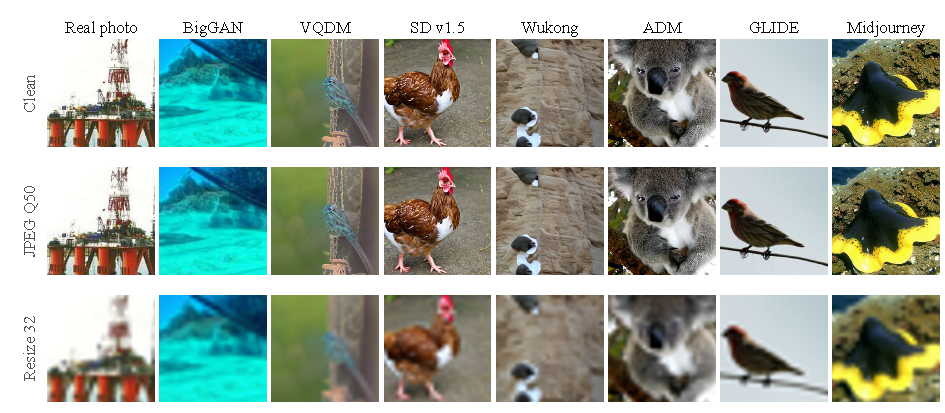
\includegraphics[width=\textwidth]{figures/examples.pdf}
\caption{One real test photo and one test image from each generator, after the shared preprocessing (shorter side 256, centre crop 224), under three of the test conditions.}\label{fig:examples}
\end{figure}

\subsection{Metrics and statistics}
The main metric is \textbf{balanced accuracy} (BA), the mean of real-photo recall and generated-image recall at the fixed threshold; with 500 images per class it equals accuracy. \textbf{AUROC} measures ranking independently of the threshold. Results are averaged over the seven held-out generators. Differences between two detectors are tested with a \textbf{paired, class-stratified bootstrap}: 2,000 resamples of each fold's test images, the same resample for both detectors, and the mean difference over folds. A difference is called significant when its 95\% percentile interval excludes zero. The intervals cover sampling of test images only; the seven folds share their real test photos, so they are not independent samples.

\subsection{Nested model selection}\label{sec:nested}
Choosing a layer, probe or fusion by its test score would leak the held-out generator into the design. We therefore choose by \emph{nested} leave-one-generator-out~\cite{varma2006bias}: inside each outer fold, every candidate is refit six times, each time with one of the six seen generators held out, and scored on that inner held-out generator. The candidate with the best inner score, averaged over the six standard conditions, is the fold's pick, and only then is it scored on the outer generator. Figure~\ref{fig:protocol} shows one outer and one inner fold.

\begin{figure}[h]
\centering
\resizebox{\textwidth}{!}{%
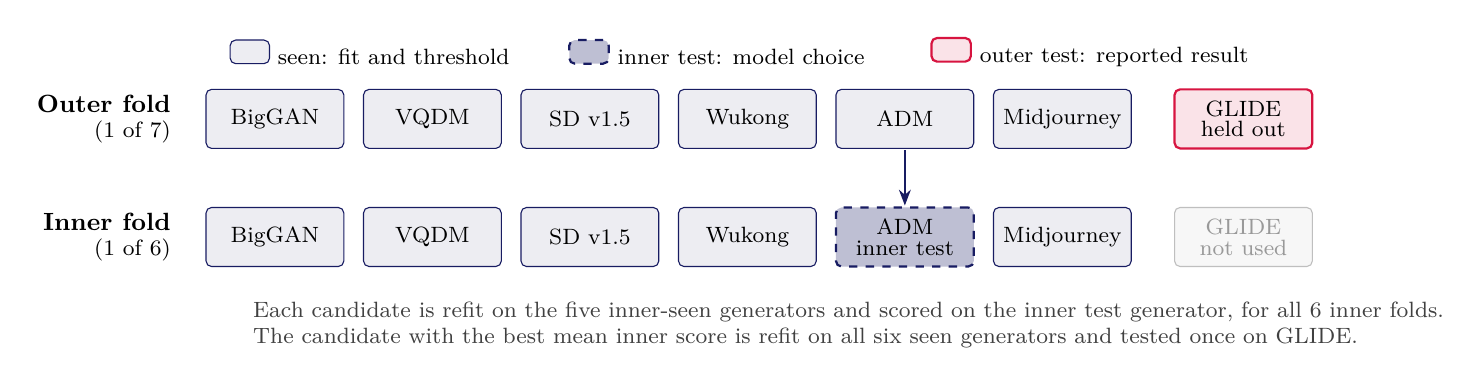
\begin{tikzpicture}[
  g/.style={draw, rounded corners=2pt, minimum width=1.75cm, minimum height=0.75cm, font=\footnotesize, align=center},
  seen/.style={g, draw=ntublue, fill=ntublue!8},
  test/.style={g, draw=ntured, thick, fill=ntured!12},
  inner/.style={g, draw=ntublue, thick, dashed, fill=ntublue!28},
  unused/.style={g, draw=black!25, text=black!40, fill=black!3},
  lab/.style={font=\small\bfseries, anchor=east, align=right}]
\def\gens{{"BigGAN","VQDM","SD v1.5","Wukong","ADM","Midjourney"}}
\node[lab] at (0.2, 0) {Outer fold\\[-2pt]{\footnotesize\mdseries (1 of 7)}};
\foreach \i in {0,...,5} \node[seen] at (1.4 + \i*2.0, 0) {\pgfmathparse{\gens[\i]}\pgfmathresult};
\node[test] at (1.4 + 6*2.0 + 0.3, 0) {GLIDE\\[-2pt]held out};
\node[lab] at (0.2, -1.5) {Inner fold\\[-2pt]{\footnotesize\mdseries (1 of 6)}};
\foreach \i in {0,1,2,3,5} \node[seen] at (1.4 + \i*2.0, -1.5) {\pgfmathparse{\gens[\i]}\pgfmathresult};
\node[inner] at (1.4 + 4*2.0, -1.5) {ADM\\[-2pt]inner test};
\node[unused] at (1.4 + 6*2.0 + 0.3, -1.5) {GLIDE\\[-2pt]not used};
\draw[-{Stealth[length=2mm]}, ntublue, thick] (1.4 + 4*2.0, -0.4) -- (1.4 + 4*2.0, -1.1);
\node[font=\footnotesize, align=left, anchor=north west, text=black!75] at (1.0, -2.2)
  {Each candidate is refit on the five inner-seen generators and scored on the inner test generator, for all 6 inner folds.\\
   The candidate with the best mean inner score is refit on all six seen generators and tested once on GLIDE.};
\node[font=\footnotesize, anchor=west] at (0.7, 0.85) {\tikz\node[seen, minimum width=0.5cm, minimum height=0.3cm]{};\ seen: fit and threshold};
\node[font=\footnotesize, anchor=west] at (5.0, 0.85) {\tikz\node[inner, minimum width=0.5cm, minimum height=0.3cm]{};\ inner test: model choice};
\node[font=\footnotesize, anchor=west] at (9.6, 0.85) {\tikz\node[test, minimum width=0.5cm, minimum height=0.3cm]{};\ outer test: reported result};
\end{tikzpicture}}
\caption{Leave-one-generator-out with nested model selection, shown for the GLIDE fold. The outer test generator is used only once, to score the chosen model. Every fold also uses real ImageNet photos: 1,600 for fitting, 400 for the threshold and 500 for the test.}\label{fig:protocol}
\end{figure}

% ================================================================== 4
\section{Methods}

\subsection{Background: the building blocks}\label{sec:background}
This section explains briefly each model and technique the experiments use; the following subsections describe how we used them.

\paragraph{Backbones.}
\begin{itemize}
  \item \textbf{ResNet-18}~\cite{he2016resnet} is an 18-layer convolutional network whose layers are linked by \emph{residual} (skip) connections, which make deep networks trainable. Pretrained on ImageNet classification, it is the standard starting point for \emph{fine-tuning}: all its weights are updated on the new task.
  \item \textbf{Vision Transformer (ViT).} A ViT cuts an image into fixed-size patches (14 or 16 pixels), embeds each as a token, adds a special \emph{CLS} token, and passes all tokens through a stack of transformer blocks (24 for the ViT-L models used here, 1024-dimensional, about 300M parameters). The CLS token's output after any block summarises the image at that depth; early blocks keep more low-level detail, late blocks more semantics.
  \item \textbf{DINOv2}~\cite{oquab2024dinov2} is a ViT-L/14 trained by \emph{self-supervised} self-distillation on 142 million curated images: a student network learns to match a teacher network's output on different crops of the same image, with no labels. Its features are general-purpose and are used here \emph{frozen}, without any weight update.
  \item \textbf{DINOv3}~\cite{simeoni2025dinov3} is DINOv2's successor, a ViT-L/16 trained the same way on 1.7 billion images, with changes that keep its patch-level features sharp.
  \item \textbf{CLIP}~\cite{radford2021clip} is a ViT-L/14 trained \emph{contrastively} on 400 million image--text pairs, so that an image's embedding is close to its caption's. UnivFD~\cite{ojha2023univfd} uses its frozen features for fake-image detection.
\end{itemize}

\paragraph{Detectors on frozen features.}
\begin{itemize}
  \item \textbf{RIGID}~\cite{he2024rigid} is training-free. It adds a little Gaussian noise to an image and measures how much the frozen DINOv2 embedding changes (cosine similarity between the two embeddings). The assumption is that real photos lie in regions of feature space that are stable under small perturbations, while generated images do not; a fixed similarity threshold decides.
  \item \textbf{Probes.} A \emph{probe} is a small classifier trained on frozen features. A \emph{linear probe} (logistic regression) learns one weight per feature dimension; an \emph{MLP probe} adds one hidden layer and can learn non-linear combinations. Only the probe is trained, so training takes seconds and the backbone cannot overfit to the training generators.
  \item \textbf{Anomaly detection} models only real photos: an image is flagged as generated when its features are far from the real-photo distribution, measured by Mahalanobis distance (distance in units of the real features' covariance) or by the distance to its $k$ nearest real neighbours.
\end{itemize}

\paragraph{Making detectors robust.}
\begin{itemize}
  \item \textbf{Data augmentation} applies the expected test-time degradations (JPEG compression, downscaling) at random to training images, so that the model learns features that survive them.
  \item \textbf{Fusion} averages the scores (logits) of two detectors after putting them on a common scale; it helps when the detectors make different errors.
  \item \textbf{Routing} uses a different detector, or threshold, for each kind of degradation; it needs to know or predict the degradation of each test image.
  \item \textbf{Threshold adaptation.} A detector outputs a score, and a threshold turns it into a decision. When degradation shifts all scores, a threshold chosen on clean images misclassifies even if the ranking of images is intact. A \emph{label-free} threshold is set from the test images themselves: we fit a mixture of two Gaussians to the scores of a batch and cut where the two components cross.
\end{itemize}

\paragraph{Evaluation.}
\begin{itemize}
  \item \textbf{Balanced accuracy} is the mean of the recall on real photos and the recall on generated images; it is not inflated by class imbalance, and 50\% is chance. \textbf{AUROC} is the probability that a random real photo scores above a random generated image; it measures ranking regardless of the threshold.
  \item \textbf{Leave-one-generator-out} cross-validation trains on all generators but one and tests on the one left out, in turn for each generator. \textbf{Nested} leave-one-generator-out repeats the same procedure inside the training generators to choose among models, so that the choice never sees the test generator.
  \item \textbf{The paired bootstrap} resamples the test images with replacement many times and recomputes the difference between two detectors on each resample; the spread of those differences gives a confidence interval.
\end{itemize}

\subsection{RIGID and probes on its features}
RIGID embeds an image $x$ and a noisy copy $x + \lambda\epsilon$ ($\epsilon \sim \mathcal{N}(0, I)$, $\lambda = 0.05$) with frozen DINOv2 ViT-L/14 and scores the image by the cosine similarity of the two embeddings; real photos are expected to score higher. As a supervised extension, a probe is trained on the clean embedding concatenated with its change under noise (\emph{clean + diff}). Real-only anomaly scores (Mahalanobis distance and $k$-nearest neighbours on real-photo features) were tried as an alternative that needs no generated images.

\subsection{Fine-tuned ResNet-18}
An ImageNet-pretrained ResNet-18~\cite{he2016resnet} with a two-class head is fine-tuned end to end: AdamW (learning rate $2\times10^{-4}$, weight decay $10^{-4}$, cosine schedule), class-weighted cross-entropy, batch size 32, 8 epochs, random resized crops (scale 0.75--1) and horizontal flips. The epoch with the best seen-validation BA is kept. An ablation adds artefact augmentation to the training images: JPEG at a random quality 30--95, a random downscale to 32, 64 or 128 pixels and back, or both, each with probability 0.5.

\subsection{Frozen DINOv2 with probes}
Images are resized (shorter side 256), centre-cropped to 224 and passed through frozen DINOv2 ViT-L/14. The CLS token, layer-normed, is the feature; for the main runs it is the final layer's, concatenated with RIGID's noise difference. Two probes are fit on standardised features:
\begin{itemize}
  \item \textbf{Logistic regression}, L2-regularised and class-balanced.
  \item \textbf{MLP}: $1024 \to 256$ (GELU, dropout 0.3) $\to 1$, trained full-batch with AdamW (learning rate $10^{-3}$, weight decay $10^{-2}$), class-balanced binary cross-entropy, and early stopping on a 10\% split (patience 20, at most 300 epochs).
\end{itemize}

\subsection{Robustness methods}
\begin{itemize}
  \item \textbf{Intermediate blocks.} The CLS token after blocks 8, 12, 16, 20 or 24 of the 24-block ViT, read with the final layer norm.
  \item \textbf{Degradation augmentation.} The ResNet study's JPEG and resize artefacts, applied to the seen generators' training images before embedding; \emph{clean + augmented} training uses the clean and the augmented embedding of every image.
  \item \textbf{Routing.} A router picks, per degradation type, the probe and threshold that are best on the seen generators' validation images degraded in the same way.
  \item \textbf{Threshold adaptation.} Besides the fixed seen-validation threshold: a label-free threshold at the crossing of a two-component Gaussian mixture fitted to an unlabelled test batch's logit scores, and the oracle threshold as an upper bound.
\end{itemize}

\subsection{Final detector and DINOv3 fusion}
Figure~\ref{fig:pipeline} shows the final detector: the block-20 MLP trained on clean + augmented images, with one threshold from clean seen validation. It needs a single image and no knowledge of how the image was degraded. For DINOv3~\cite{simeoni2025dinov3} we use ViT-L/16 (timm's copy of the LVD-1689M weights) at 224 pixels, read the same blocks, and \emph{fuse} two MLPs by averaging their logits after standardising each on clean seen validation.

\begin{figure}[h]
\centering
\resizebox{\textwidth}{!}{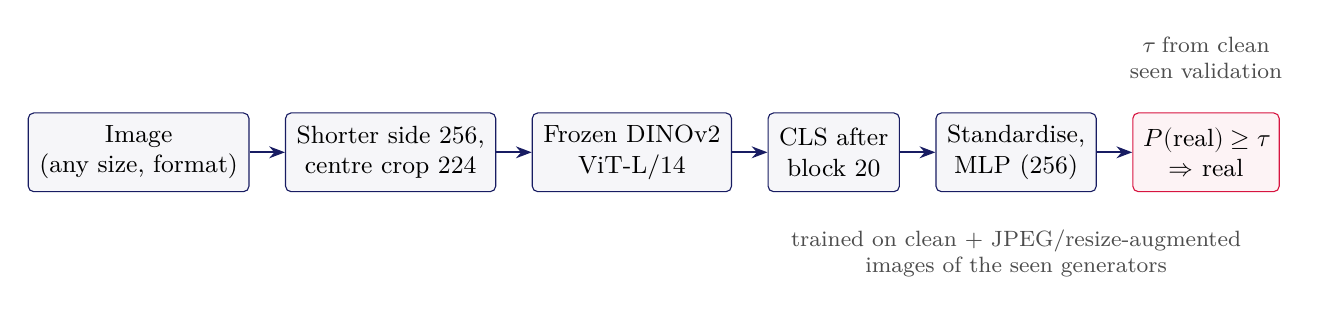
\begin{tikzpicture}[
  box/.style={draw=ntublue, rounded corners=2pt, align=center, font=\small, minimum height=1.0cm, inner sep=4pt, fill=ntublue!4},
  arr/.style={-{Stealth[length=2mm]}, ntublue, thick}, node distance=0.45cm]
\node[box] (img) {Image\\(any size, format)};
\node[box, right=of img] (pre) {Shorter side 256,\\centre crop 224};
\node[box, right=of pre] (vit) {Frozen DINOv2\\ViT-L/14};
\node[box, right=of vit] (cls) {CLS after\\block 20};
\node[box, right=of cls] (mlp) {Standardise,\\MLP (256)};
\node[box, right=of mlp, draw=ntured, fill=ntured!5] (dec) {$P(\text{real}) \ge \tau$\\$\Rightarrow$ real};
\foreach \a/\b in {img/pre, pre/vit, vit/cls, cls/mlp, mlp/dec} \draw[arr] (\a) -- (\b);
\node[font=\footnotesize, text=black!70, below=0.35cm of mlp, align=center] {trained on clean + JPEG/resize-augmented\\images of the seen generators};
\node[font=\footnotesize, text=black!70, above=0.3cm of dec, align=center] {$\tau$ from clean\\seen validation};
\end{tikzpicture}}
\caption{The final detector. Only the 263k-parameter MLP is trained; the 300M-parameter backbone is frozen.}\label{fig:pipeline}
\end{figure}

% ================================================================== 5
\section{Results}

\subsection{Overview: the research path}\label{sec:path}
The experiments were not planned in advance as a grid. Each one answered a question raised by the previous result, and most of them either tested whether an apparent gain was real or tried to fix the weakness the last step had exposed. Table~\ref{tab:path} summarises the path; the subsections that follow take each step in turn, starting with what motivated it and ending with what it led to.

\begin{table}[h]
\centering\footnotesize
\caption{The research path. M = Michael Yip Hoi Weng, T = Tyrone Tiang Jin Shen, S = Choi Seunghwan.}\label{tab:path}
\renewcommand{\arraystretch}{1.25}
\begin{tabularx}{\textwidth}{@{}>{\raggedright\arraybackslash}p{2.6cm}>{\raggedright\arraybackslash}X>{\raggedright\arraybackslash}X>{\raggedright\arraybackslash}p{3.0cm}@{}}
\toprule
Step & Question & Answer & Led to \\
\midrule
1. RIGID and its probes (M) \S\ref{sec:res-rigid} & Can a frozen model detect fakes with no training? Does a little supervision fix it? & Sometimes: AUROC 0.96--0.99 on FFHQ, about 0.5 on COCO. A probe reaches 0.90--0.93 on an unseen generator, but 0.65--0.76 on a new dataset. & Train on fakes, but measure generalisation under control. \\
2. ResNet-18 vs frozen DINOv2 (T, S) \S\ref{sec:res-baselines} & How does a fine-tuned CNN transfer, and do frozen features do better on the same protocol? & ResNet 72.2\% clean over 7 holdouts; frozen DINOv2 MLP 85.3\%, ahead by 9--22\pp\ everywhere. & Is 85\% real? \\
3. Stress tests (S) \S\ref{sec:res-stress} & Family leakage, file-format shortcut, seed noise? & Each costs a little; the headline survives at about 84\%. & It breaks under degradation: 61.6\% at 32 pixels. \\
4. Robustness (S, T's augmentation) \S\ref{sec:res-robust} & Routing, augmentation, better features? & Routing and augmentation +1.5--1.7\pp; block 20 +3.3\pp\ clean; a 22-probe router 79.2\%. & Were these choices real, or picked on the test generators? \\
5. Nested selection (S) \S\ref{sec:res-nested} & Does seen-generator validation pick the right model? & No, it rewards overfitting. Nested selection confirms block 20. & Is the remaining loss in the features or the threshold? \\
6. Thresholds (S) \S\ref{sec:res-threshold} & How much of the degradation loss is threshold drift? & For block 20, most of it: a label-free threshold gives 80.2\%. & Fix the drift in training instead. \\
7. Final detector (S) \S\ref{sec:res-final} & Block 20 + augmented training; can one fixed threshold work? & Yes: 81.3\% on single images, +20.5\pp\ over the ResNet. & Can another backbone or more pixels beat it? \\
8. CLIP blocks, native resolution (S) \S\ref{sec:res-negative} & Do intermediate CLIP blocks or native-resolution tiles help? & CLIP reads JPEG as ``real''; native tiles lean on image size. Neither survives the controls. & A stronger self-supervised backbone. \\
9. DINOv3 (S) \S\ref{sec:res-dinov3} & Does DINOv2's successor help without a shortcut? & On GenImage, yes: fusion 84.4\% (+3.1\pp), format check passed. & Test outside GenImage. \\
10. CIFAKE (S) \S\ref{sec:res-cifake} & Does the ranking hold on another dataset? & No: final detector 76.5\%, fusion 70.7\%. & Keep the final detector; test at full resolution. \\
\bottomrule
\end{tabularx}
\end{table}

\subsection{RIGID: strong on some sources, near chance on others}\label{sec:res-rigid}
\why{A detector that needs no generated images cannot overfit to the generators it was trained on, so a training-free method is the natural first try for unseen generators.}
Without training, RIGID reaches AUROC 0.957--0.990 on FFHQ (LDM, StyleGAN2) and 0.867 on Unsplash vs Stable Diffusion, but only 0.49--0.59 on COCO with SD3, SD3.5 and Midjourney 6, 0.52 on ImageNet DiT and 0.57 on LSUN-ADM. A diagnostic sweep over preprocessing (squashing, cropping, native resolution, matched sizes, JPEG round trips) shows that its score depends strongly on resolution and compression. A probe on clean + diff features lifts AUROC to 0.94--0.98 on unseen images of the training datasets and about 0.90--0.93 on an unseen generator of the same dataset, but only 0.65--0.76 on a different dataset. A probe trained on ImageNet and Synthbuster together reaches 0.80--0.90 on new collections (COCO, Unsplash, and LSUN/FFHQ/DiT/GigaGAN). Real-only anomaly detection, which models only real photos and so cannot be biased towards seen generators, was no better than RIGID (AUROC 0.77, 0.56 and 0.88 against RIGID's 0.77, 0.54 and 0.87).
\ledto{The noise-stability signal is real but not universal, and some supervision with generated images is needed. That makes generalisation to an unseen generator the central risk, and it needs a controlled benchmark in which only the generator changes: the protocol of Section~\ref{sec:protocol}.}

\subsection{Fine-tuned ResNet-18 vs frozen DINOv2}\label{sec:res-baselines}
\why{A standard supervised baseline, evaluated on the strict protocol, sets the bar. Running every other detector on exactly the same splits, thresholds and test images then makes every later comparison paired, image by image.}
With GLIDE held out, the fine-tuned ResNet reaches 85.1\% BA on clean images but 56.7\% at JPEG Q50 and 50--51\% at 64 and 32 pixels. Augmentation helps only the degradation it imitates (Table~\ref{tab:resnet}): JPEG augmentation lifts JPEG Q50 to 76.0\% at almost no clean cost, while resize augmentation helps downscaling but costs 9.4\pp\ clean.

\begin{table}[h]
\centering\small
\caption{ResNet-18 with GLIDE held out: balanced accuracy by training augmentation.}\label{tab:resnet}
\begin{adjustbox}{max width=\textwidth}\begin{tabular}{lrrrr}
\toprule
Test condition & Baseline & JPEG only & Resize only & JPEG + resize \\
\midrule
Clean & \best{85.1} & 84.3 & 75.7 & 73.2 \\
JPEG Q50 & 56.7 & \best{76.0} & 56.6 & 67.8 \\
Resize 128 & 70.8 & 60.3 & \best{73.8} & 71.2 \\
Resize 64 & 51.0 & 51.0 & 66.4 & \best{67.5} \\
Resize 32 & 50.3 & 50.2 & 61.7 & \best{63.3} \\
128 + JPEG 50 & \best{61.8} & 56.3 & 58.8 & 61.7 \\
\bottomrule
\end{tabular}\end{adjustbox}
\end{table}

Over all seven holdouts the picture is worse (Table~\ref{tab:logo}). The ResNet averages 72.2\% clean, from 55.3\% on VQDM to 90.4\% on GLIDE, although it scores 86\% on the seen generators' validation images. On the same splits, a frozen DINOv2 MLP on clean + diff features reaches 85.3\% clean and beats the ResNet by 9--22\pp\ in every condition, all significant. Re-scoring the ResNet checkpoints reproduces the published numbers to within 0.1\pp, so the comparison is image for image. Averaging the two models' logits is worse than DINOv2 alone in every condition ($-2.0$\pp\ clean, $-16.5$\pp\ at 64 pixels).

The test-time view matters for the ResNet. Its published sweep squashes each image to 224$\times$224, while the GLIDE ablation, like DINOv2, centre-crops it. On the same checkpoints, squashing is better by 2.3\pp\ clean and 9.9\pp\ at 128 pixels, because training used random resized crops that show most of the image. The GLIDE figures of Table~\ref{tab:resnet} (85.1\%) and of the sweep (90.4\%) come from two different training runs that also picked different epochs; on one checkpoint the two views differ by only 1.2\pp.
\ledto{The ResNet scores 86\% on the seen generators but 72\% on unseen ones: the first sign of a theme that recurs throughout, that fit to seen generators is not generalisation. Frozen features with a small head become the reference, and its 85.3\% headline is tested next.}

\begin{table}[h]
\centering\small
\caption{Mean balanced accuracy (\%) over the seven held-out generators.}\label{tab:logo}
\begin{adjustbox}{max width=\textwidth}\begin{tabular}{lrrrrrr}
\toprule
Detector & Clean & JPEG Q50 & Resize 128 & Resize 64 & Resize 32 & 128+JPEG \\
\midrule
ResNet-18, fine-tuned & 72.2 & 63.3 & 66.4 & 51.7 & 52.4 & 59.0 \\
RIGID (no training) & 75.9 & 69.1 & 70.3 & 57.3 & 50.0 & 54.4 \\
DINOv2, logistic regression (clean) & 80.5 & \best{74.8} & 77.9 & 73.1 & \best{63.8} & \best{70.1} \\
DINOv2, MLP (clean + diff) & \best{85.3} & 74.7 & \best{81.5} & \best{74.1} & 61.6 & 68.1 \\
\bottomrule
\end{tabular}\end{adjustbox}
\end{table}

\subsection{Stress tests of the headline}\label{sec:res-stress}
\why{Before building on 85.3\%, rule out the obvious ways it could be inflated: related generators on both sides of the split, a file-format cue, and luck in training.}
\begin{itemize}
  \item \textbf{Family leakage.} SD v1.5 and Wukong are both Stable Diffusion models, so holding out one still trains on the other. Holding out the whole family costs 2.9--5.8\pp\ on them; ADM and GLIDE, also siblings, do not help each other. Holding out every generator's family lowers the MLP's mean to 84.2\% ($-1.1$\pp).
  \item \textbf{File-format shortcut.} Every GenImage real photo is a high-quality JPEG; every generated image is a PNG of a fixed size. When both classes go through the same pipeline (Format 256+q96), the MLP drops to 82.5\% ($-2.8$\pp): generated recall falls from 83\% to 72\%, so JPEG-compressed fakes look real. Midjourney drops most, from 78.1\% to 68.6\%. Training on format-aligned images recovers most of this (84.8\%). The fine-tuned ResNet loses only 0.7\pp.
  \item \textbf{Seed noise.} Over five training seeds the standard deviation of the seven-generator mean is 0.2--0.4\pp, and every key comparison keeps its sign on every seed.
\end{itemize}
Figure~\ref{fig:sizes} shows why format and size are risky in GenImage: the two classes differ in both, so a detector can separate them without looking at what the image shows.

\begin{figure}[h]
\centering
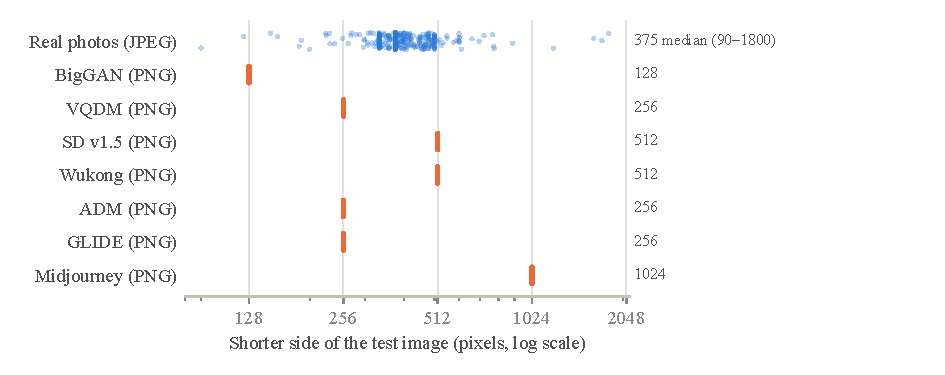
\includegraphics[width=\textwidth]{figures/sizes.pdf}
\caption{Shorter side of the test images, by class (500 per row; one dot per image). Every generator produces one fixed size and saves PNG files; the real photos are JPEGs of varied size. Both properties carry the label.}\label{fig:sizes}
\end{figure}
\ledto{The headline survives at about 84\%, and the format-matched test becomes a standard check for every later detector. The real weakness is degradation: 74.7\% at JPEG Q50 and 61.6\% at 32 pixels. That is the next problem.}

\subsection{Robustness to JPEG and resizing}\label{sec:res-robust}
\why{The clean + diff MLP is best on clean images but the clean-only logistic regression degrades least, which suggested choosing a probe per degradation. Tyrone's ablation suggested augmentation. And DINOv2's last layer may simply not be the best one to read.}

\paragraph{Routing and augmentation.} Picking the probe per degradation type on degraded seen validation raises the mean over the six conditions from 74.2\% to 75.7\%; predicting the degradation from the image itself (83\% accurate) keeps 75.4\%. Training the final-layer MLP on clean + augmented images gives a similar +1.7\pp\ with one detector.

\paragraph{Intermediate blocks.} The choice of layer matters far more (Table~\ref{tab:layers}, Figure~\ref{fig:layers}). Blocks 12--16 reach 95--97\% on seen validation but collapse to about 50--56\% under JPEG: they overfit the seen generators' artefacts. Block 20 combines the two regimes: 88.6\% clean (+3.3\pp\ over the final layer) and +4.3 to +4.8\pp\ under resizing. CLIP ViT-L/14, the UnivFD backbone, is strong on clean images (87.7\%) but loses 10--17\pp\ under every degradation. Averaging the logits of the DINOv2 and CLIP MLPs gives the best clean result, 90.0\%, but CLIP pulls it down under degradation. A router choosing among all 22 frozen-feature probes on degraded seen validation averages 79.2\% over the six conditions (+5.0\pp), picking block-20 and multi-layer probes for most conditions.

\begin{table}[h]
\centering\small
\caption{Frozen-feature MLPs by layer, clean training (mean BA over the 7 holdouts, \%). Seen val = accuracy on the seen generators' validation images.}\label{tab:layers}
\begin{adjustbox}{max width=\textwidth}\begin{tabular}{lrrrrrr}
\toprule
Features & Clean & JPEG Q50 & Resize 64 & Resize 32 & Format 256+q96 & Seen val \\
\midrule
DINOv2 final layer, clean + diff & 85.3 & 74.7 & 74.1 & 61.6 & 82.5 & 89.9 \\
DINOv2 block 12 & 83.6 & 53.1 & 52.8 & 50.0 & 67.5 & \best{97.0} \\
DINOv2 block 16 & 85.3 & 56.6 & 55.9 & 50.9 & 76.9 & 96.7 \\
DINOv2 block 20 & \best{88.6} & 74.7 & \best{78.5} & \best{66.4} & \best{83.4} & 94.6 \\
DINOv2 block 24 & 81.5 & \best{76.9} & 74.4 & 66.1 & 80.3 & 85.5 \\
CLIP ViT-L/14 & 87.7 & 63.9 & 57.4 & 51.1 & 74.6 & 93.4 \\
\bottomrule
\end{tabular}\end{adjustbox}
\end{table}

\begin{figure}[h]
\centering
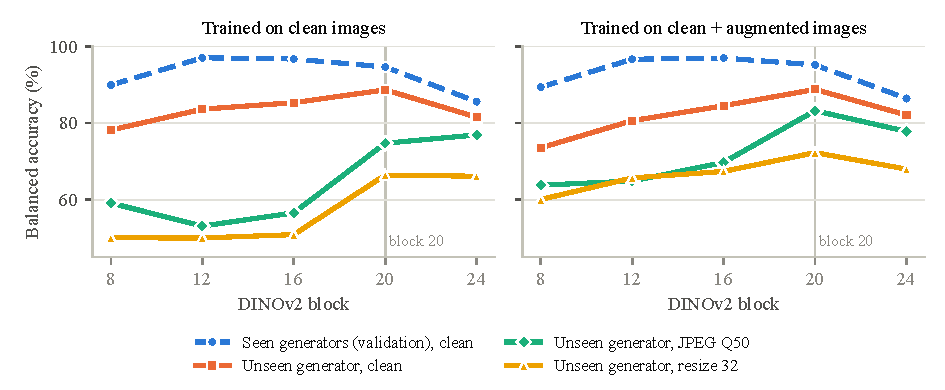
\includegraphics[width=\textwidth]{figures/layers.pdf}
\caption{DINOv2 MLP probes by block (mean BA over the 7 folds). Left: on clean training, accuracy on the seen generators (dashed) peaks at blocks 12--16, exactly where the unseen generator under JPEG or at 32 pixels collapses towards chance; block 20 is best on unseen generators. Right: augmented training lifts the degraded curves, most at block 20 (Section~\ref{sec:res-final}).}\label{fig:layers}
\end{figure}

\ledto{The layer matters far more than routing or augmentation on the final layer. But block 20 and the CLIP fusion were spotted on the test generators, and seen-generator validation would have picked the fragile blocks 12--16. The choices had to be re-made honestly.}

\subsection{Nested model selection}\label{sec:res-nested}
\why{Three results showed seen-generator validation misleading: it ranked blocks 12--16 first, it ranked the ResNet + DINOv2 ensemble first, and it made the 22-probe router pick a block-12 probe for clean ADM, scoring 67\% there. Nested leave-one-generator-out (Section~\ref{sec:nested}) chooses by accuracy on a seen generator held out from a refit, which mirrors the real task.}

The nested scores rank candidates almost exactly as the outer test does (block 20 on clean images: 87.2\% inner, 88.6\% outer; the CLIP fusion 88.9\% and 90.0\%). For clean images, nested selection picks the DINOv2 + CLIP fusion in 4 of 7 folds, an honest +2.3\pp\ over the main MLP against the post-hoc +4.7\pp\ of always using it. Over the six conditions it picks block 20 or the block-24 mean-patch probe, and with thresholds adapted block 20 is the clear first choice. A nested router reaches 78.8\%, level with the 22-probe router (79.2\%), and fixes its clean-ADM failure (67\% $\to$ 77\%). Selecting on clean seen validation instead picks the fragile early blocks and loses 6.9\pp.
\ledto{Block 20 is a legitimate choice, not luck, and accuracy on the seen generators is not a proxy for generalisation; this is the clearest methodological lesson of the project. Under degradation, though, block 20's AUROC fell much less than its balanced accuracy, which pointed at the threshold.}

\subsection{Threshold drift vs lost information}\label{sec:res-threshold}
\why{Under degradation AUROC falls much less than BA, so part of the loss may be a threshold tuned on clean images that no longer separates the classes, rather than information destroyed by the degradation.}
For the final-layer MLP, little of it is: even the oracle threshold recovers only 2.2\pp. For block 20, a lot is: the oracle recovers 10--15\pp\ at JPEG Q50. Figure~\ref{fig:drift} (top row) shows why: under JPEG Q50 the two classes stay largely separable, but the generated images' scores slide to the right, past the fixed threshold. The label-free Gaussian-mixture threshold lands within 0.6--0.8\pp\ of the oracle and lifts block 20 to 80.2\% over the six conditions, more than the 22-probe router (79.2\%), without knowing the degradation, and holds at 78.7--79.7\% on batches that are 20\% or 80\% real. The ResNet's collapse at 64 and 32 pixels is not a threshold problem: its oracle reaches only 53--55\%.
\ledto{Block 20 keeps the information but its scores shift. A label-free threshold needs a batch of images that share one degradation, so the next step was to remove the drift in training instead, so that one fixed threshold works on single images.}

\subsection{The final detector}\label{sec:res-final}
\why{Combine the two strongest findings, block-20 features and augmented training, and test whether single-image thresholds can replace the batch threshold.}
Combining block 20 with augmented training gives the final detector (Table~\ref{tab:final}). Augmentation, worth +1.7\pp\ on the final layer, is worth +4.6\pp\ on block 20, with +8.5\pp\ at JPEG Q50 and +10.0\pp\ at 128 + JPEG and no clean cost: block 20 still carries the fine detail the probe can learn to read under degradation. Augmentation also removes most of the threshold drift (Figure~\ref{fig:drift}, bottom row): the fixed threshold is within 2.1\pp\ of the oracle, so thresholds read from file metadata (size, JPEG quality) add only 0.3\pp\ and condition-aware routers add nothing.

\begin{figure}[h]
\centering
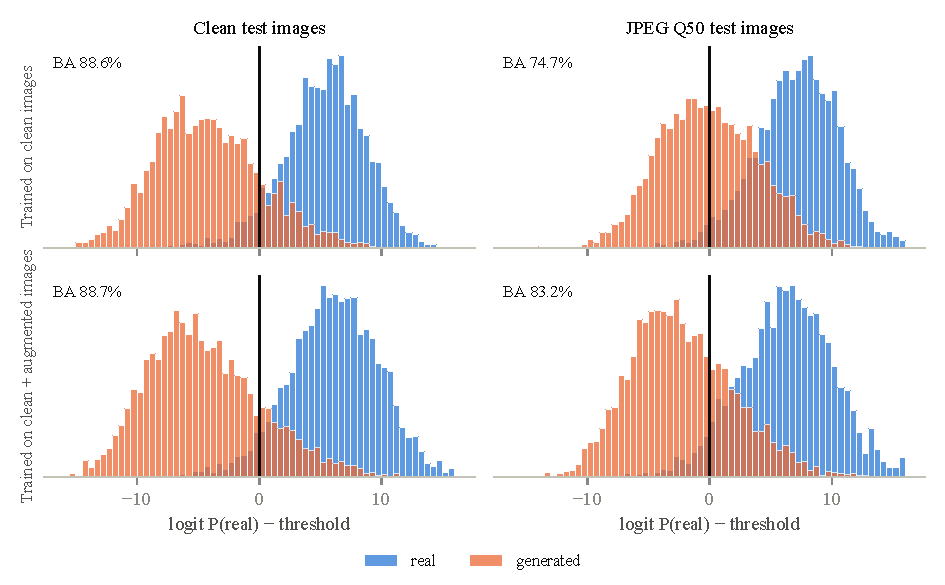
\includegraphics[width=\textwidth]{figures/drift.pdf}
\caption{Block-20 MLP scores on the held-out generator's test images, relative to the fixed threshold (0 = threshold; right of it = called real), pooled over the 7 folds; values beyond $\pm16$ are drawn at the edge. Top: trained on clean images, JPEG Q50 shifts the generated images' scores past the threshold. Bottom: with augmented training the generated images stay on the left.}\label{fig:drift}
\end{figure}

\begin{table}[h]
\centering\small
\caption{The final detector (mean BA over the 7 holdouts, \%). Mean = over the six standard conditions.}\label{tab:final}
\setlength{\tabcolsep}{4.5pt}
\begin{adjustbox}{max width=\textwidth}\begin{tabular}{lrrrrrrr}
\toprule
Detector & Clean & JPEG Q50 & Resize 64 & Resize 32 & 128+JPEG & Format & Mean \\
\midrule
ResNet-18, fine-tuned & 72.2 & 63.3 & 51.7 & 52.4 & 59.0 & 71.5 & 60.8 \\
DINOv2 final-layer MLP (main runs) & 85.3 & 74.7 & 74.1 & 61.6 & 68.1 & 82.5 & 74.2 \\
Block-20 MLP, clean training & 88.6 & 74.7 & 78.5 & 66.4 & 66.3 & 83.4 & 76.7 \\
\textbf{Block-20 MLP, clean + augmented} & 88.7 & 83.2 & 80.7 & 72.3 & 76.4 & 85.5 & \textbf{81.3} \\
\quad with label-free batch threshold & \best{90.5} & \best{86.2} & \best{81.6} & \best{72.8} & \best{78.0} & \best{89.0} & \best{82.9} \\
\bottomrule
\end{tabular}\end{adjustbox}
\end{table}

The final detector works on single images, needs neither the degradation type nor metadata, and averages 81.3\%: +7.1\pp\ over the main runs' DINOv2 MLP and +20.5\pp\ over the fine-tuned ResNet. When images arrive in batches that share one degradation, the label-free threshold adds 1.6\pp. Nested selection over all 32 clean and augmented layer probes picks either this detector or an augmented concatenation of blocks 12--24 (81.2\% vs 81.3\%, not significant); augmentation also removes the early blocks' fragility, lifting the concatenation from 70.2\% to 82.2\%. Figure~\ref{fig:conditions} summarises the progression, and Figure~\ref{fig:generators} shows it per generator: ADM and Midjourney remain the hardest. Tables~\ref{tab:pergen} and~\ref{tab:pergen6} in Appendix~\ref{app:pergen} give the per-generator numbers, clean and averaged over the six conditions.
\ledto{Two directions remained untried: a second backbone, whose intermediate blocks might behave like DINOv2's, and more pixels, since every detector so far sees a 224-pixel crop of a downscaled image.}

\begin{figure}[h]
\centering
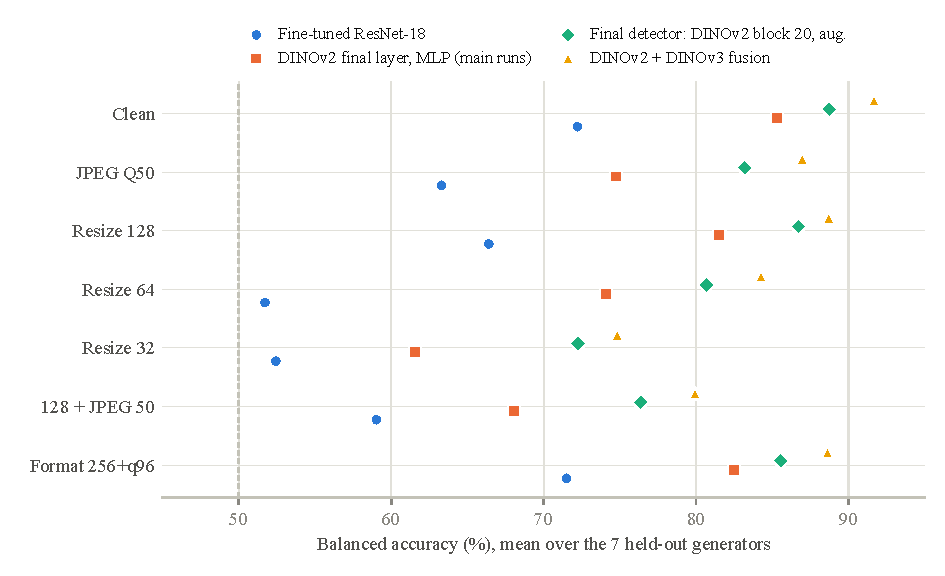
\includegraphics[width=\textwidth]{figures/conditions.pdf}
\caption{Mean balanced accuracy over the seven held-out generators, per test condition. The dashed line is chance. Each step from the fine-tuned ResNet to the final detector helps most under degradation.}\label{fig:conditions}
\end{figure}

\begin{figure}[h]
\centering
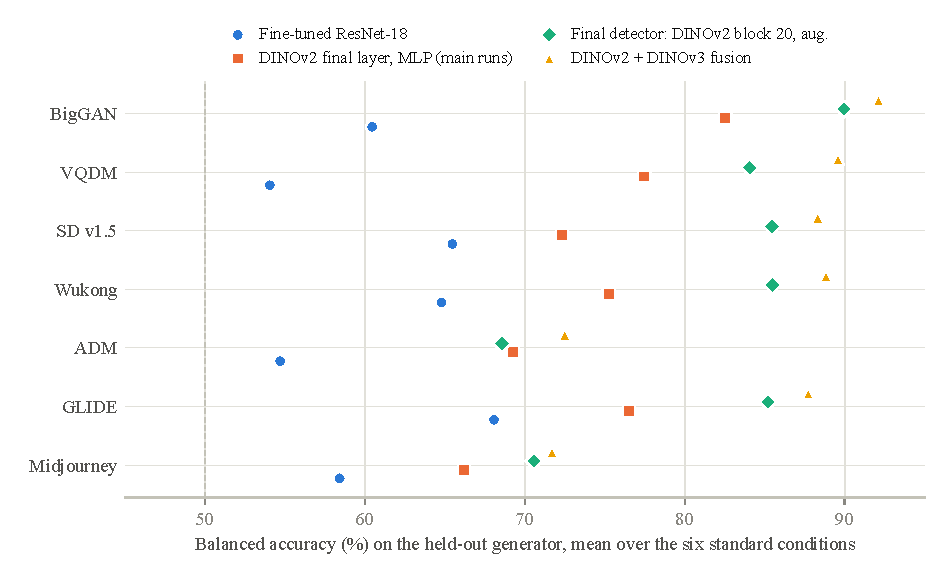
\includegraphics[width=\textwidth]{figures/generators.pdf}
\caption{Balanced accuracy on each held-out generator, mean over the six standard conditions.}\label{fig:generators}
\end{figure}

\subsection{What did not help: CLIP blocks and native resolution}\label{sec:res-negative}
\why{Intermediate DINOv2 blocks beat its final layer; perhaps the same holds for CLIP, the UnivFD backbone. And downscaling discards most of the pixels of large images, which may hold the finest generator artefacts.}

\paragraph{Intermediate CLIP blocks.} CLIP block 16 reaches 92.1\% clean, the best single feature found, but on the format-matched test it falls to 59--67\%: generated recall drops from 86\% to 18--34\%, because it reads JPEG compression as ``real''. Fusing CLIP with the final detector adds about 1\pp, and the fusion that nested selection prefers loses 3.0\pp\ on the format-matched test. The six standard conditions cannot detect this shortcut, because none of them removes the PNG/JPEG difference.

\paragraph{Native resolution.} Every detector sees a 224-pixel crop of a downscaled image. Averaging DINOv2 over up to four native-resolution 224-pixel tiles gains +4.4\pp\ clean and +5.0\pp\ format-matched; under JPEG Q50 it loses 2.6\pp, with AUROC unchanged, the threshold drift of Section~\ref{sec:res-threshold}. But image size differs by class in GenImage (real photos about 375$\times$500; generated images 128--1024 pixels), so the probe could be learning ``content at photo scale means real''. When every image is first resized to the same shorter side (448), only +2.8\pp\ clean survives, and $-0.2$\pp\ on the format-matched test. The native tile mean also recognises small real photos less often than typical ones (93.6\% vs 98.1\%), the signature of a size cue.
\ledto{About 1--3\pp\ of the native-resolution gain is genuine detail; the rest was a size cue, and CLIP's gain was a format cue. Both new directions failed the same way, because every shortcut in GenImage favours one class. A stronger version of the backbone that already worked was the remaining option.}

\subsection{DINOv3 fusion}\label{sec:res-dinov3}
\why{CLIP and native resolution failed the shortcut checks. DINOv3, DINOv2's successor trained on 1.7 billion images, is the natural next backbone.}
DINOv3 was run through the same pipeline: blocks 8--24, clean and augmented training, 24 candidates, nested selection. In all seven folds nested selection picks the fusion of the final detector with a DINOv3 block-24 MLP (Table~\ref{tab:dinov3}). It is significantly better in every condition (+2.0 to +3.8\pp) and on every held-out generator (+1.1\pp\ on Midjourney to +5.5\pp\ on VQDM). Unlike CLIP, it passes the format check: clean to format-matched costs it 3.1\pp, the same as the final detector, and generated recall on the format-matched test rises from 74\% to 80\%. DINOv3's own blocks behave like DINOv2's: block 20 is the best single block, and clean-only training drifts under JPEG until augmentation fixes it.
\ledto{The fusion is the strongest detector on GenImage by every measure there. Before replacing the final detector, it had to be tested on a dataset outside GenImage.}

\begin{table}[h]
\centering\small
\caption{DINOv3 (mean BA over the 7 holdouts, \%; all trained on clean + augmented images). $\Delta$ = fusion minus final detector, paired bootstrap; * = 95\% interval excludes 0.}\label{tab:dinov3}
\setlength{\tabcolsep}{4.5pt}
\begin{adjustbox}{max width=\textwidth}\begin{tabular}{lrrrrrrr}
\toprule
Detector & Inner & Clean & JPEG Q50 & Resize 32 & 128+JPEG & Format & Mean \\
\midrule
Final detector (DINOv2 block 20) & 80.6 & 88.7 & 83.2 & 72.3 & 76.4 & 85.5 & 81.3 \\
\textbf{Fusion with DINOv3 block 24} & \best{83.8} & 91.7 & 87.0 & \best{74.8} & \best{79.9} & 88.6 & \best{84.4} \\
DINOv3 block 20, logistic regression & 82.5 & \best{93.9} & \best{87.4} & 71.3 & 76.8 & \best{90.0} & 83.7 \\
DINOv3 block 24, MLP & 80.8 & 89.9 & 84.1 & 71.3 & 75.9 & 87.6 & 81.2 \\
\midrule
$\Delta$ fusion $-$ final & & +2.9* & +3.8* & +2.6* & +3.6* & +3.1* & +3.1* \\
\bottomrule
\end{tabular}\end{adjustbox}
\end{table}

\subsection{Cross-dataset test: CIFAKE}\label{sec:res-cifake}
\why{All selection so far, nested or not, happened inside GenImage. Only a different dataset can show whether the GenImage ranking holds.}
Both detectors were retrained on all seven generators, with the threshold calibrated on held-out real photos and every generator's validation images, and scored on CIFAKE's test split: 10,000 CIFAR-10 photos and 10,000 Stable Diffusion v1.4 images, all 32$\times$32 JPEGs, so the format is matched by construction (Table~\ref{tab:cifake}, Figure~\ref{fig:cifake}).

\begin{table}[h]
\centering\small
\caption{CIFAKE test split. BA at the threshold shipped from GenImage, at the label-free Gaussian-mixture threshold of the test set, and at the oracle threshold. The DINOv3 head's scores are recovered from the fusion as $2z_{\text{fused}} - z_{\text{DINOv2}}$.}\label{tab:cifake}
\begin{adjustbox}{max width=\textwidth}\begin{tabular}{lrrrrr}
\toprule
Detector & AUROC & BA shipped & BA label-free & BA oracle & Real / gen.\ recall \\
\midrule
Final detector (DINOv2 block 20) & \best{0.853} & \best{76.5} & \best{76.7} & \best{77.1} & 71 / 82 \\
DINOv2 + DINOv3 fusion & 0.835 & 70.7 & 75.5 & 75.6 & 52 / 89 \\
DINOv3 block-24 head alone & 0.709 & & & 65.4 & \\
\bottomrule
\end{tabular}\end{adjustbox}
\end{table}

\begin{figure}[h]
\centering
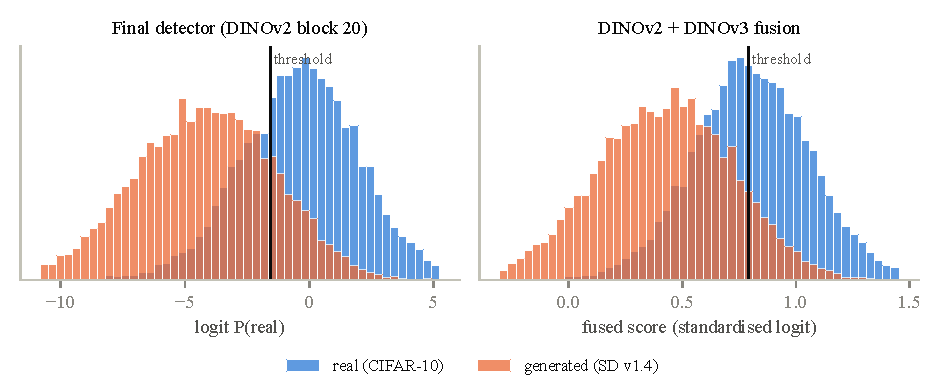
\includegraphics[width=\textwidth]{figures/cifake_scores.pdf}
\caption{Score distributions on CIFAKE. The final detector's shipped threshold sits near the valley between the classes; the fusion's threshold sits inside the real-photo peak, so it calls about half of the real photos generated.}\label{fig:cifake}
\end{figure}

The final detector transfers better than its GenImage 32-pixel result (72.3\%) would suggest: 76.5\%, with the GenImage threshold within 0.6\pp\ of the best possible one. The fusion, better on every GenImage condition, is worse here. Its DINOv3 head is weak on these images (AUROC 0.709), and its scores drift so that only 52\% of real photos are called real; a label-free threshold recovers most of the drift but not the ranking. The GenImage ranking of the two best detectors therefore reverses on the first dataset outside GenImage. CIFAKE is one dataset with one generator at a tiny size, close to the SD v1.5 images in training, so it tests new real photos and extreme downscaling more than a new generator.
\ledto{The final detector stays the DINOv2 block-20 MLP. The fusion remains a candidate until it also wins on full-resolution external sets with newer generators (Section~\ref{sec:conclusion}).}

% ================================================================== 6
\section{Discussion}

\subsection{Shortcuts in GenImage}
Three properties of GenImage separate the classes without any generator artefact: file format (JPEG photos vs PNG fakes), image size (each generator has one fixed size, real photos vary), and the resampling that follows from size. Each new direction we tried exploited one of them: the base detector the format (about 2--3\pp), CLIP's intermediate blocks the format (up to 33\pp), native-resolution tiles the size (about 2\pp). None of the six standard conditions removes these cues, so a detector chosen on them, even by careful nested selection, can still be choosing a shortcut. The format-matched and size-matched controls were what exposed each case; we regard them as necessary checks for any new feature.

\subsection{Model selection must use a held-out generator}
Seen-generator validation repeatedly pointed the wrong way: it ranked the fragile early DINOv2 blocks first (95--97\% seen vs 50--56\% under JPEG on unseen generators), ranked the ResNet + DINOv2 ensemble first although it is worse than DINOv2 alone, and led a router to a block-12 probe that scores 97\% on seen generators and 67\% on ADM. Nested leave-one-generator-out selection, which mirrors the deployment problem, ranked candidates almost exactly as the real test did. Its limit appeared with DINOv3: nested selection inside GenImage is still selection for GenImage, and the CIFAKE test reversed its choice.

\subsection{Limitations}
\begin{itemize}
  \item \textbf{One benchmark for training.} All GenImage results share ImageNet real photos and 2021--2023 generators. The only cross-dataset test of the final detectors, CIFAKE, is at 32 pixels.
  \item \textbf{Statistical scope.} One data split and one real-photo source; the seven folds share their real test photos; bootstrap intervals cover image sampling only.
  \item \textbf{Batch thresholds.} The label-free threshold needs a batch of unlabelled images that share one degradation. The single-image detector does not, which is why it is the final detector.
  \item \textbf{Researcher choices.} DINOv3 was tried after CLIP and native resolution had failed; this adds a small selection effect that the nested protocol does not measure. DINOv3's training data is not public and could contain images from these generators.
\end{itemize}

% ================================================================== 7
\section{Conclusion and Future Work}\label{sec:conclusion}
A small MLP on a frozen intermediate block of DINOv2, trained on JPEG- and resize-augmented images of known generators, detects images from an unseen generator with 81.3\% mean balanced accuracy over six degradations from a single image and a single threshold, against 60.8\% for a fine-tuned ResNet-18 and 74.2\% for the same probe on the final layer. The gain comes mainly from choosing the right layer and training it on degraded images, and it survives nested selection, family hold-outs and format-matched tests. A DINOv3 fusion is better still on GenImage (84.4\%) but worse on CIFAKE, so the final detector remains the DINOv2 block-20 MLP.

The main open question is transfer beyond GenImage. Both detectors are exported with a scoring script, and the next step is to test them on full-resolution external sets with newer generators, such as Synthbuster~\cite{bammey2023synthbuster} with RAISE photos and COCO with SD3 and Midjourney 6. Training with random rescaling, so that size and resampling carry no label, is the most promising way to remove the remaining size cue.

% ------------------------------------------------------------------ references
\begin{thebibliography}{99}\small
\bibitem{bammey2023synthbuster} Q.~Bammey. Synthbuster: Towards detection of diffusion model generated images. \emph{IEEE Open Journal of Signal Processing}, 5, 2024.
\bibitem{bird2024cifake} J.~J.~Bird and A.~Lotfi. CIFAKE: Image classification and explainable identification of AI-generated synthetic images. \emph{IEEE Access}, 12, 2024.
\bibitem{grommelt2024fake} P.~Grommelt, L.~Weiss, F.-J.~Pfreundt and J.~Keuper. Fake or JPEG? Revealing common biases in generated image detection datasets. \emph{arXiv:2403.17608}, 2024.
\bibitem{he2016resnet} K.~He, X.~Zhang, S.~Ren and J.~Sun. Deep residual learning for image recognition. In \emph{CVPR}, 2016.
\bibitem{he2024rigid} Z.~He, P.-Y.~Chen and T.-Y.~Ho. RIGID: A training-free and model-agnostic framework for robust AI-generated image detection. \emph{arXiv:2405.20112}, 2024.
\bibitem{ojha2023univfd} U.~Ojha, Y.~Li and Y.~J.~Lee. Towards universal fake image detectors that generalize across generative models. In \emph{CVPR}, 2023.
\bibitem{oquab2024dinov2} M.~Oquab, T.~Darcet, T.~Moutakanni et al. DINOv2: Learning robust visual features without supervision. \emph{Transactions on Machine Learning Research}, 2024.
\bibitem{radford2021clip} A.~Radford, J.~W.~Kim, C.~Hallacy et al. Learning transferable visual models from natural language supervision. In \emph{ICML}, 2021.
\bibitem{simeoni2025dinov3} O.~Sim\'eoni, H.~V.~Vo, M.~Seitzer et al. DINOv3. \emph{arXiv:2508.10104}, 2025.
\bibitem{varma2006bias} S.~Varma and R.~Simon. Bias in error estimation when using cross-validation for model selection. \emph{BMC Bioinformatics}, 7:91, 2006.
\bibitem{wang2020cnn} S.-Y.~Wang, O.~Wang, R.~Zhang, A.~Owens and A.~A.~Efros. CNN-generated images are surprisingly easy to spot\ldots\ for now. In \emph{CVPR}, 2020.
\bibitem{zhu2023genimage} M.~Zhu, H.~Chen, Q.~Yan et al. GenImage: A million-scale benchmark for detecting AI-generated image. In \emph{NeurIPS Datasets and Benchmarks Track}, 2023.
\end{thebibliography}

% ------------------------------------------------------------------ appendix
\clearpage
\appendix
\sloppy
\section{Per-Generator Results}\label{app:pergen}
Table~\ref{tab:pergen} gives each held-out generator's clean balanced accuracy and AUROC for the main detectors, and Table~\ref{tab:pergen6} their balanced accuracy averaged over the six standard conditions. The fine-tuned ResNet fails on VQDM, ADM and Midjourney; every frozen-feature detector finds ADM and Midjourney hardest.

\begin{table}[H]
\centering\small
\caption{Clean balanced accuracy (\%) and AUROC on each held-out generator.}\label{tab:pergen}
\setlength{\tabcolsep}{4pt}
\begin{adjustbox}{max width=\textwidth}\begin{tabular}{lrrrrrrrr}
\toprule
Detector & BigGAN & VQDM & SD v1.5 & Wukong & ADM & GLIDE & Midj. & Mean \\
\midrule
ResNet-18, fine-tuned & 75.7 & 55.3 & 79.8 & 79.4 & 61.6 & 90.4 & 63.3 & 72.2 \\
DINOv2 final-layer MLP & 92.8 & 86.1 & 85.6 & 86.5 & 76.6 & 91.5 & 78.1 & 85.3 \\
Final detector & 97.1 & 92.3 & 92.1 & 92.4 & 72.9 & \best{96.1} & 78.3 & 88.7 \\
DINOv2 + DINOv3 fusion & \best{97.8} & \best{96.7} & \best{95.7} & \best{95.4} & \best{77.3} & 95.3 & \best{83.5} & \best{91.7} \\
\midrule
\multicolumn{9}{l}{\emph{AUROC}} \\
ResNet-18, fine-tuned & 0.869 & 0.633 & 0.878 & 0.875 & 0.689 & 0.971 & 0.703 & 0.803 \\
Final detector & 0.998 & 0.977 & 0.978 & 0.979 & 0.876 & 0.994 & 0.909 & 0.959 \\
DINOv2 + DINOv3 fusion & 0.999 & 0.994 & 0.992 & 0.992 & 0.908 & 0.996 & 0.948 & 0.976 \\
\bottomrule
\end{tabular}\end{adjustbox}
\end{table}

\begin{table}[H]
\centering\small
\caption{Balanced accuracy (\%) on each held-out generator, mean over the six standard conditions.}\label{tab:pergen6}
\setlength{\tabcolsep}{4pt}
\begin{adjustbox}{max width=\textwidth}\begin{tabular}{lrrrrrrrr}
\toprule
Detector & BigGAN & VQDM & SD v1.5 & Wukong & ADM & GLIDE & Midj. & Mean \\
\midrule
ResNet-18, fine-tuned & 60.4 & 54.0 & 65.5 & 64.8 & 54.7 & 68.1 & 58.4 & 60.8 \\
DINOv2 final-layer MLP & 82.5 & 77.5 & 72.3 & 75.2 & 69.3 & 76.5 & 66.2 & 74.2 \\
Final detector & 90.0 & 84.0 & 85.4 & 85.5 & 68.6 & 85.2 & 70.6 & 81.3 \\
DINOv2 + DINOv3 fusion & \best{92.1} & \best{89.6} & \best{88.3} & \best{88.8} & \best{72.5} & \best{87.7} & \best{71.7} & \best{84.4} \\
\bottomrule
\end{tabular}\end{adjustbox}
\end{table}

\section{Reproduction}
All code, result files and the exported detectors are in the project repository (branch \texttt{seunghwan/dinov2-genimage-holdout}); every number in this report is copied from a result file under \texttt{results/}. The main entry points:
\begin{itemize}
  \item \texttt{scripts/train\_resnet\_generalization.py}: ResNet-18 training and evaluation for one held-out generator.
  \item \texttt{scripts/dinov2\_genimage\_holdout.py --held-out all}: RIGID and DINOv2 probes on all seven folds; \texttt{scripts/summarize\_logo.py} averages them.
  \item \texttt{scripts/backbone\_features.py}, \texttt{scripts/augmented\_backbone\_features.py}: block-wise DINOv2 (and CLIP) features of clean, augmented and degraded images.
  \item \texttt{scripts/nested\_selection\_experiments.py}, \texttt{scripts/augmented\_layer\_selection.py}: nested leave-one-generator-out selection.
  \item \texttt{scripts/final\_detector\_experiments.py}: the final detector and its threshold rules.
  \item \texttt{scripts/clip\_layer\_features.py --backbone dinov3} and \texttt{scripts/clip\_layer\_experiments.py --backbone dinov3}: the DINOv3 experiments.
  \item \texttt{scripts/export\_final\_detector.py [--detector fusion]} and \texttt{scripts/score\_final\_detector.py [--fusion]}: export the detectors and score any folders of images, as in the CIFAKE test.
  \item \texttt{report/make\_figures.py}: the figures of this report.
\end{itemize}

\section{Team Contributions}
\begin{itemize}
  \item \textbf{Michael Yip Hoi Weng}: RIGID, the training-free starting point; probes on RIGID features; real-only anomaly detection; cross-dataset tests of RIGID and its probes (CIFAKE, Synthbuster/RAISE, COCO, Unsplash, FFHQ/LSUN).
  \item \textbf{Tyrone Tiang Jin Shen}: the fine-tuned ResNet-18 baseline, the leave-one-generator-out protocol and its test conditions, the augmentation ablation and the seven-generator sweep.
  \item \textbf{Choi Seunghwan}: frozen DINOv2 detectors on the shared protocol; stress tests (family leakage, format shortcut, seeds); robustness (routing, augmentation, intermediate blocks, threshold adaptation); nested model selection; the final detector; CLIP, native-resolution and DINOv3 experiments; export and the CIFAKE test.
\end{itemize}

\end{document}
